%%%%%%%%%%%%%%%%%%%%%%%%%%%%%%%%%%%%%%%%%%%%%%%%%%%%%%%%%%%%
% Pedro Brandao's trial to get a template for thesis for students
% Used the upthesis from Fernando Silva (see upthesis).
% See also the packages file.
% 2014/07/07 First draft
% 2014/07/21 
%  pbrandao: added the list of listings (it should produce portuguese name if
%           babel is set to portuguese, see packages.tex). Changed usepackage of babel
%           to be before input packages.tex to allow test

%
%%%%%%%%%%%%%%%%%%%%%%%%%%%%%%%%%%%%%%%%%%%%%%%%%%%%%%%%%%%%
% LTeX: language=portuguese

% makes all pages the height of the text on that page. No extra vertical space is added.
\raggedbottom 
% setting it to report will remove the blank pages before each chapter
\documentclass[11pt,a4paper,twoside]{book}


%%%%%%%%%%%%%%%%%%%%%%%%%%%%%%%%%%%%%%%%%%%%%%%%%%%%%%%%%%%%
%%%   Packages that need to be configured for the thesis
%%%%%%%%%%%%%%%%%%%%%%%%%%%%%%%%%%%%%%%%%%%%%%%%%%%%%%%%%%%%

% Language settings
% use UKenglish for UK or leave blank for US English
% it will also change the names for some of the chapters (list of tables, figures, content,
%\usepackage[UKenglish]{babel}
%\usepackage[portuguese]{babel}
% If you have multiple languages (as in this text) you can use both, leaving last the main one.
% Then you can use 
% \begin{otherlanguage}{UKenglish}
% text in other language, UKEnglish in this case
% \end{otherlanguage}
\usepackage[UKenglish]{babel}


%%%%%%%%%%%%%%%%%%%%%%%%%%%%%%%%%%%%%%%%%%%%%%%%%%%%%%%%%%%%
%%%   Packages uses language definitions
% see file below for more packages and settings
%%%%%%%%%%%%%%%%%%%%%%%%%%%%%%%%%%%%%%%%%%%%%%%%%%%%%%%%%%%%
\usepackage{upthesis}
\usepackage{xcolor}

% the bibliography file
\addbibresource{refs.bib}


%% Definitions for acronyms
\newcommand*\acronymbiggest{HTTP} % defines the biggest Acronym used to define the column size



\usepackage[
%backref={section},
%pagebackref, % for getting references to the page where the citation is (in the biblio), note that biblatex above also has this
pdfpagelabels=false
]{hyperref}
\hypersetup{pdftitle={Test}, %nao suporta acentos
   pdfkeywords ={palavras chave},
   pdfsubject = {assunto},
	bookmarksnumbered=true,
   pdfauthor ={Your name}, % see other options on manual (can be page) needs empty line on bibitem
   plainpages=false, 
   pdfborder={0 0 0},
   colorlinks,%colorlinks=false,
   breaklinks=true,
	%hyperindex=true 	% Makes the page numbers of index entries into hyperlinks. Relays on unique page anchors (pageanchor) 
% see for colors http://mirror.ctan.org/macros/latex/contrib/xcolor/xcolor.pdf
   linkcolor=	Sepia, %MidnightBlue,% BlueViolet,%Sepia, % Color for normal internal links.
   %anchorcolor=black,% Color for anchor text.
   citecolor=RedViolet,% Color for bibliographical citations in text.
   %filecolor=cyan% Color for URLs which open local files.
   %menucolor=red% Color for Acrobat menu items.
   %runcolor=filecolor% Color for run links (launch annotations).
   urlcolor=NavyBlue% Color for linked URLs.
}
%use the same style for \url as the text
% from http://en.wikibooks.org/wiki/LaTeX/Hyperlinks#Customization
\urlstyle{same}

\usepackage{tikz}
\usetikzlibrary{automata,positioning}


\begin{document}

\title{Thesis title}
%% The following is not currently being used.
% Part of the coverp in upthesis.sty
% \submitionplace{Tese submetida à Faculdade de Ciências da \\
%   Universidade do Porto para obtenção do grau de Mestre \\ 
%   em Ciência de Computadores}
% \author{Nome do autor}
% \department{Departamento de Ciência de Computadores \\ Faculdade de
%   Ciências da Universidade do Porto}
% \submitdate{Setembro 2015}


\beforepreface%



\prefacesection{Abstract}

Hey, this is the abstract of my thesis. It should be a brief summary of the work, highlighting the main objectives, methods, results, and conclusions. The abstract should be concise and informative, allowing readers to quickly understand the essence of the research.
\textbf{Keywords:} key, word.


\prefacesection{Resumo}
O teu resumo COOL, its me TEST WOWIEESSS

\textbf{Palavras-chave:} palavra, chave..


\prefacesection{Acknowledgements}

First of all, I would like to thank my family, etc, etc
\dedicationpage{Dedico à minha mãe \ldots}



% end of thesis preamble
\afterpreface%

%% main tex here
%% By putting the chapter names here, one can just comment the content in the chapters 
%% and produce a pdf with the correct chapter number.
%% If you want further configurability you can use subfiles package
%% https://www.ctan.org/pkg/subfiles

%\chapter{Introduction}\label{chap:intro}
\chapter{Introduction}\label{chap:intro}

%https://www.usenix.org/system/files/sec22-turonova.pdf
%https://arxiv.org/abs/2407.20479
%https://www.regular-expressions.info/catastrophic.html

In this chapter, the problem is overviewed, the study's importance is explained along with goals for the proposed solution. 

\section{Background}
Regular expressions are a foundational tool in computer science, widely used in pattern matching, lexical analysis, input validation, and string processing. Their expressiveness and concise syntax make them a powerful language for describing regular languages.

% However, when implemented without care, especially in backtracking-based engines, regular expressions can become a source of serious security vulnerabilities.

A regular expression $R$ is used (along with an input $W$) in regex matching engines. The matching engines will verify if $W$ is fully matched by $R$, meaning that the entire input is a match - or they will verify if a substring of $W$ is matched by $R$. 

% Current matching engines commonly fall into one of the following categories:
% \begin{itemize}
% 	\item \textbf{Finite State Machine Regular Expression Engines}: A finite state machine (or finite \emph{automaton}) is built and evaluated using every symbol $\sigma \in W$. Used \emph{UNIX}-based systems.
% 	\item \textbf{Backtracking Regular Expression Engines}: Instead of building a finite state machine, 
% \end{itemize}

\section{Regular Expression Denial of Service}
One such vulnerability is known as \emph{Regular Expression Denial of Service} (ReDoS). ReDoS exploits the pathological worst-case behavior of certain regular expressions, causing exponential time complexity during matching. In typical backtracking matchers---such as those found in JavaScript, Java, and many scripting environments---ambiguous or nested expressions (especially involving repetition, such as \texttt{(a+)+}) can lead the engine to explore an exponential number of paths for certain crafted inputs. This behavior allows an attacker to intentionally supply inputs that force excessive computation, effectively rendering a service unavailable or degraded.

The root of the ReDoS problem lies not in regular expressions as a theoretical model but in how they are operationalized in software. While deterministic finite automata (DFAs) evaluate regular expressions in linear time, many real-world engines opt for backtracking NFAs due to their flexibility and ease of implementation. Unfortunately, these NFAs are susceptible to exponential blow-up in ambiguous or unguarded patterns.

\section{}

\chapter{Preliminaries}\label{chap:prelim}
Theory builds upon theory, therefore it is essential to establish a solid foundation by understanding the basic concepts and terminology that compose the core topics of formal languages and automata theory.
In this chapter we begin by formally defining what a language is and then move on to describe the class of languages known as regular languages.
Along the way, we will also introduce various concepts such as finite automata (DFA, NFA) and regular expressions.

\section{Alphabets, Strings, and Languages}
\subsection*{Alphabets}

An \emph{alphabet} is a finite, non-empty set of symbols, typically denoted by the Greek letter $\Sigma$. That is,
\[
\Sigma = \{ a_1, a_2, \dots, a_n \}
\]

\noindent where each $a_i$ is a symbol in the alphabet.

For example, one can represent the binary alphabet as $\Sigma = \{ 0, 1 \}$, or the English alphabet as $\Sigma = \{ a, b, c, \ldots, z \}$.

\subsection*{Strings}
A \emph{string} over an alphabet $\Sigma$ is a finite sequence of symbols from $\Sigma$. Strings are typically denoted by $w$, and the \emph{length} of a string $w$ is denoted by $|w|$.

The set of all strings over the alphabet $\Sigma$ is denoted by $\Sigma^*$ and defined as:
\[
\Sigma^* = \{ w \mid w \text{ is a finite sequence of symbols from } \Sigma \}
\]

The unique string of length zero is called the \emph{empty string}, denoted by $\varepsilon$.
It is important to note that $\varepsilon \in \Sigma^*$.

For example, if $\Sigma = \{ 0, 1 \}$, then we have that:
\begin{center}
	$\Sigma^* = \{ \varepsilon, 0, 1, 00, 01, 10, 11, 000, 001, 010, 011, 100, 101, 110, 111, \ldots \}$
\end{center}

Where the empty string is, as mentioned above, denoted by $\varepsilon$ and also belongs to $\Sigma^*$.

\subsection*{Languages}

A \emph{language} over an alphabet $\Sigma$ is a set of strings over $\Sigma$.

\[
L \subseteq \Sigma^*
\]

That is, a language is any subset of $\Sigma^*$, possibly infinite, finite, or even empty. \newline
Since a language is a set of strings, the following standard set operations can be applied (assuming $A$ and $B$ are languages over the same alphabet $\Sigma$):

\begin{itemize}
	\item \emph{Intersection}: $A \cap B = \{ x \mid x \in A \text{ and } x \in B \}$
	\item \emph{Union}: $A \cup B = \{ x \mid x \in A \text{ or } x \in B \}$
	\item \emph{Difference}: $A \setminus B = \{ x \mid x \in A \text{ and } x \notin B \}$
\end{itemize}

Furthermore, we can also operate specifically over languages with the following operations (assuming $L_1$ and $L_2$ are languages over the same alphabet $\Sigma$):

\begin{itemize}
	\item \emph{Concatenation}: $L_1 \cdot L_2 = \{ xy \mid x \in L_1 \text{ and } y \in L_2 \}$
	\item \emph{Kleene Star}: $L^* = \bigcup_{n=0}^{\infty} L^n$, where $L^0 = \{\varepsilon\}$ and $L^n = L \cdot L^{n-1}$ for $n > 0$.
	\item \emph{Reversal}: $L^R = \{ x^R \mid x \in L \}$, where $x^R$ denotes the reversal of string $x$.
	\item \emph{Complement}: $\overline{L} = \Sigma^* - L$, i.e., the set of all strings over $\Sigma$ that are not in $L$.
\end{itemize}

These operations form the basis for reasoning about the expressiveness and closure properties of language classes such as regular, context-free, and context-sensitive languages. In particular, regular languages are closed under all the operations listed above, including union, intersection, concatenation, and Kleene star. This robustness makes them especially amenable to algorithmic manipulation, as seen in finite automata and regular expression engines.

\section{Finite Automata}
A \emph{finite automaton} is a model of computation used to recognize regular languages. It processes input strings symbol by symbol and determines whether the string belongs to the language defined by the automaton. There are two main types of finite automata:

\begin{itemize}
    \item \textbf{Deterministic Finite Automaton (DFA)}: An automaton where, for each state and input symbol, there is exactly one possible next state.
    \item \textbf{Non-deterministic Finite Automaton (NFA)}: An automaton that allows multiple possible transitions for a given state and input symbol, including transitions without consuming any input (called $\varepsilon$-transitions).
\end{itemize}

Formally defined, an NFA is a 5-tuple $(Q, \Sigma, \delta, Q_0, F)$ where:

\begin{itemize}
    \item $Q$ is a finite set of states,
    \item $\Sigma$ is the input alphabet,
    \item $\delta: Q \times (\Sigma \cup \{\varepsilon\}) \rightarrow 2^Q$ is the transition function,
    \item $Q_0 \subseteq Q$ is the set of initial states,
    \item $F \subseteq Q$ is the set of accepting (final) states.
\end{itemize}

A string $w \in \Sigma^*$ is accepted by the NFA if there exists a sequence of transitions (possibly including $\varepsilon$-moves) that consumes $w$ and ends in a state $q$ such that $q \in F$.

\begin{figure}[H]
	\centering
	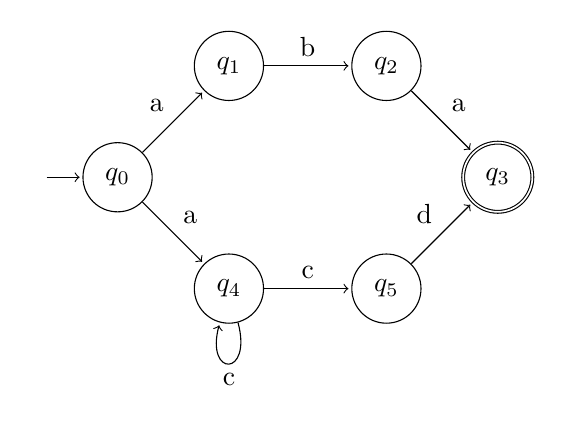
\begin{tikzpicture}[shorten >=1pt,node distance=2cm,on grid,auto,initial text=]
		\node[state, initial] (q0) {$q_0$};
		\node[state] (q1) [above right=of q0] {$q_1$};
		\node[state] (q2) [right=of q1] {$q_2$};
		
		\node[state] (q4) [below right=of q0] {$q_4$};
		\node[state] (q5) [right=of q4] {$q_5$};
		
		\node[state, accepting] (q3) [below right=of q2] {$q_3$};
		
		\path[->]
		(q0) edge node {a} (q1)
			 edge node {a} (q4)
		
		(q1) edge node {b} (q2)
		
		(q2) edge node {a} (q3)

		(q4) edge node {c} (q5)
		 	 edge[loop below] node {c} ()
		
		(q5) edge node {d} (q3);
	\end{tikzpicture}
	\caption{Example of an NFA that accepts $L = \{aba, a(c^*)d\}$}
\label{fig:nfa_example}
\end{figure}



An NFA is \emph{deterministic} (also known as DFA) if $|\delta(q,\sigma)| \leq 1$, for any $(q,\sigma) \in Q \times \Sigma$ and $|Q_0| = 1$.

\begin{figure}[H]
\centering
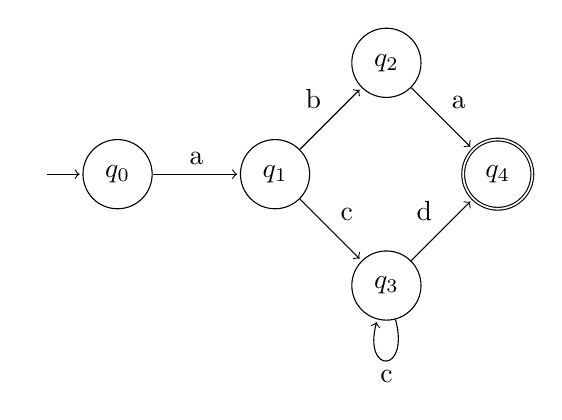
\begin{tikzpicture}[shorten >=1pt,node distance=2cm,on grid,auto,initial text=]
	\node[state, initial] (q0) {$q_0$};
	\node[state] (q14) [right=of q0] {$q_1$};
	\node[state] (q2) [above right=of q14] {$q_2$};
	\node[state] (q45) [below right=of q14] {$q_3$};
	\node[state, accepting] (q3) [above right=of q45] {$q_4$};

    \path[->]
    	(q0) edge node {a} (q14)
    	
    	(q14) edge node {b} (q2)
    		  edge node {c} (q45)
    	
    	(q2) edge node {a} (q3)
    	
    	(q45) edge[loop below] node {c} (q45)
    		  edge node {d} (q3);
  
\end{tikzpicture}
\caption{A DFA whose language is the same as the NFA from figure \ref{fig:nfa_example}} 
\end{figure}

\section{Regular Expressions}
Let $\Sigma$ be a finite alphabet. Let $L \subseteq \Sigma$. The set of \emph{regular expressions} over $\Sigma$, denoted by $\text{RegExp}(\Sigma)$, is defined inductively as follows:

\begin{itemize}
    \item $\emptyset$ is a regular expression denoting the empty language: $L(\emptyset) = \emptyset$.
    \item $\varepsilon$ is a regular expression denoting the language containing only the empty string: $L(\varepsilon) = \{ \varepsilon \}$.
    \item For each symbol $a \in \Sigma$, $a$ is a regular expression denoting the singleton language: $L(a) = \{ a \}$.
    \item If $r_1$ and $r_2$ are regular expressions, then so are:
    \begin{itemize}
        \item $(r_1 \mid r_2)$, denoting the union: $L(r_1 \mid r_2) = L(r_1) \cup L(r_2)$.
        \item $(r_1 \cdot r_2)$, denoting concatenation: $L(r_1 \cdot r_2) = L(r_1) \cdot L(r_2)$.
        \item $(r_1)^*$, denoting Kleene star: $L(r_1^*) = (L(r_1))^*$.
    \end{itemize}
\end{itemize}

For each $r \in \text{RegExp}(\Sigma)$, the function $L(r)$ yields the language defined by $r$.

Parentheses are used to disambiguate expressions and enforce precedence; by convention, Kleene star binds most tightly ($a^*$), followed by concatenation (e.g. $a \cdot b$, whose operator "$\cdot$" is omitted for convenience), and finally union ($+$).

We denote by $\alpha = \beta$ if two regular expressions $\alpha$ and $\beta$, both over $\Sigma$, represent the same language ($L(\alpha) = L(\beta)$).
Furthermore, if both expressions can be decomposed in a way that they still represent the same language, they are denoted by $\alpha \equiv \beta$.

If the language of a regular expression $\alpha$ contains the empty word, then that regular expression possesses the \textit{empty word property}.

\begin{defn}[Empty Word Property]
	The empty word property is characterized by the function $\varepsilon : \text{RegExp} \rightarrow \{ \varepsilon, \emptyset \}$ and is defined recursively as follows, given $\alpha$ and $\beta$ regular expressions defined over $\Sigma$:
	\begin{gather*}
		\varepsilon(\emptyset) = \emptyset \\
		\varepsilon(\varepsilon) = \varepsilon \\
		\varepsilon(a) = \emptyset, \: a \in \Sigma \\
		\varepsilon(\alpha + \beta) = \begin{cases}
			\emptyset & \text{if $\varepsilon(\alpha) = \varepsilon(\beta) = \emptyset$} \\
			\varepsilon & \text{if $\varepsilon(\alpha) = \varepsilon$ or $\varepsilon(\beta) = \varepsilon$}
		\end{cases} \\
		\varepsilon(\alpha \beta) = \begin{cases}
			\emptyset & \text{if $\varepsilon(\alpha) = \emptyset$ or $\varepsilon(\beta) = \emptyset$} \\
			\varepsilon & \text{if $\varepsilon(\alpha) = \varepsilon(\beta) = \varepsilon$}
		\end{cases} \\
		\varepsilon(a^*) = \varepsilon
	\end{gather*}
\end{defn}




%	\varepsilon(\alpha + \beta) = \begin{cases}
	%		
	%	\end{cases}

%	\varepsilon(\alpha + \beta) &= \emptyset \\
%	\varepsilon(\alpha + \beta), \; \text{if } \varepsilon(\alpha)\text{=}\varepsilon(\beta)\text{=}\emptyset 

%One can see if the language of a regular expression contains the empty word by utilizing the \textit{empty word property}, which is defined as the function $\varepsilon : RegExp \rightarrow \{\varepsilon, \emptyset\}$. \\
%Given $\alpha,\beta \in \text{RegExp}(\Sigma)$ and $a \in \Sigma$,



	
\subsection{Extended Regular Expressions}
\label{chap:prelim:extended_re}
In addition to the basic operations, some other operators are often used for convenience. These include:

\begin{itemize}
    \item \textbf{Kleene plus}: Given a regular expression $r$, the expression $r^+$ denotes one or more repetitions of $r$:
    \[
    L(r^+) = L(r) \cdot L(r)^*.
    \]

    \item \textbf{Fixed repetition (power)}: For a regular expression $r$ and integer $n \geq 0$, the expression $r^n$ denotes $n$ consecutive concatenations of $r$:
    \[
    L(r^0) = \{ \varepsilon \}, \quad L(r^n) = L(r) \cdot L(r^{n-1}) \text{ for } n > 0.
    \]

	 \item \textbf{Bounded repetition}: For a regular expression $r$ and integers $m, n$ with $0 \leq m \leq n-1$, the bounded repetition $r^{[m,n]}$ denotes the language containing all strings formed by concatenating between $m$ and $n-1$ copies of strings from $L(r)$:
    \[
    L(r^{[m,n]}) = \bigcup_{k=m}^{n-1} L(r^k).
    \]
\end{itemize}

These forms do not increase the expressive power of regular expressions but are useful for readability and practical applications. They can always be rewritten using the fundamental operators: union and concatenation.

\subsection{Derivatives}
\label{chap:prelim:derivatives}
% Need 1962 Janusz Brzozowski's paper for this section
The \emph{derivative of a regular expression} was first introduced in 1962 by Janusz Brzozowski. It is a powerful concept used to define the behavior of regular expressions in a more operational manner. They can be used as a means of verifying equivalence of regular expressions, for example. The derivative of a regular expression $r$ with respect to a symbol $a$ is another regular expression $d_a(r)$ that describes the set of strings that can be obtained by taking the derivative of $r$ with respect to $a$.

\begin{defn}[Derivative of a Regular Expression \cite{brzozowski_derivatives}]
	The derivative of a regular expression $r$ with respect to $\sigma \in \Sigma$ is itself a regular expression $d_\sigma(r)$ such that $\mathcal{L}(d_\sigma(r)) = \{w \ \vert \ \sigma w \in \mathcal{L}(r)\}$ and is defined as:
	\begin{align*}
		& d_\sigma(\emptyset) = \emptyset \\
		& d_\sigma(\varepsilon) = \emptyset \\
		& d_\sigma(r') = \begin{cases}
			\varepsilon & \text{if $\sigma' = \sigma$} \\
			\emptyset & \text{otherwise,}
		\end{cases} \\
		& d_\sigma(r+r') = d_\sigma(r)+d_\sigma(r') \\
		& d_\sigma(rr') = \begin{cases}
			d_\sigma(r)r' & \text{if $\varepsilon(r) = \emptyset$} \\
			d_\sigma(r)r' + d_\sigma(r') & \text{otherwise,}
		\end{cases} \\
		& d_\sigma(r^*) = d_\sigma(r)r^* \\
		& d_\sigma(r^+) = d_\sigma(r)r^*
	\end{align*}
\end{defn}


Brzozowski defined a DFA equivalent to a regular expression with the help of derivatives. With this, it is important to note that, for example, a regular expression $r = a^*$ (matches zero or more 'a' symbols) can be used to construct an equivalent DFA using Brzozowski's construction, even though $d_a(r) = a \cdot d_a(r)$ may look like it can lead to an infinite construction.

\begin{defn} [\cite{brzozowski_derivatives}]
	Two regular expressions are similar if one can be transformed to the other using only the identities:
	
	\begin{align*}
		& R + R = R, \\
		& P + Q = Q + P, \\
		& (P + Q) + R = P + (Q + R) \\
		& \varepsilon R = R \varepsilon= R \\
		& \emptyset R = R \emptyset = \emptyset
	\end{align*}
	
	Two regular expressions are dissimilar if and only if they are not similar.
\end{defn}

With this, Brzozowski proved in \cite[Theorem 5.2]{brzozowski_derivatives} that every regular expression has only a finite number of dissimilar derivatives. The big disadvantage is that, as he stated, the resulting automaton is far from minimal.

\subsection{Partial Derivatives}
The notion of \textit{partial derivative} was introduced by Antimirov \cite{pdregex_antimirov}. Opposite to Brzozowski's derivatives, \textit{partial derivatives} will lead to the construction of an NFA.

Let $\alpha \in RegExp(\Sigma)$ be a \textit{regular expression} over $\Sigma$. The set of partial derivatives of $\alpha$ with respect to a symbol $b \in \Sigma$, represented as $\partial_b(\alpha)$, is defined as follows:

\begin{align*}
	\partial_b(\emptyset) &= \emptyset		&	\partial_b(\alpha + \beta) &= \partial_b(\alpha) \cup \partial_b(\beta), \; \beta \neq \alpha \\
	\partial_b(\varepsilon) &= \emptyset	&	\partial_b(\alpha \beta) &= \partial_b(\alpha)\beta \cup \partial_b(\beta), \; \text { if } \varepsilon(\alpha) = \varepsilon \\
	\partial_b(b) &= \varepsilon & \partial_b(\alpha \beta) &= \partial_b(\alpha)\beta, \; \text { if } \varepsilon(\alpha) = \emptyset \\
	\partial_b(c) &= \emptyset, \; b \neq c \text{ and } b \in \Sigma & \partial_b(\alpha^*) &= \partial_b(\alpha)\alpha^*
\end{align*}

The set of partial derivatives by a word $w \in \Sigma^*$ 

For instance, given the regular expression $r = (ad + d^*)db$, where $\Sigma = \{a,b,d\}$, the set of partial derivatives of $r$ for the symbol $d$ is given by
\begin{align*}
	\partial_d(r) &= \partial_d((ad + d^*)db) \\
	&= \partial_d(addb + d^*db) \\
	&= \partial_d(addb) \, \cup \, \partial_d(d^*db) \\
	&= \partial_d(a)ddb \, \cup \, \partial_d(d^*)db \, \cup \, \partial_d(db) \\
	&= \emptyset ddb \, \cup \, \partial_d(d)d^*db \, \cup \, \partial_d(d)b \, \cup \, \partial_d(b) \\
	&= \emptyset \, \cup \, d^*db \, \cup \, b \, \cup \, \emptyset
\end{align*}
resulting in $\partial_d(r) = \{d^*db, b\}$.

\subsubsection{Linear Form}
\label{chap:prelim:linear_form}
It is possible to calculate the partial derivatives for every symbol $a \in \Sigma$ of a regular expression $r$ over $\Sigma$ in a single pass. To do this, Antimirov \cite{pdregex_antimirov} defined the \emph{linear form}.

A linear form $lf$ of a regular expression $\alpha$ is a finite set of symbol–continuation pairs.  
These pairs are called \textit{monomials} and they can encode all the possible one-symbol prefixes of that regular expression.

Formally, given an alphabet $\Sigma$ and the set of all regular expressions over $\Sigma$ denoted $RegExp$, a monomial is an element of $\Sigma \times RegExp$.
We denote the set of all monomials for a given alphabet $\Sigma$ by $M_\Sigma$.
  
A \emph{linear form} is then a finite set of monomials:
\[
lf(\alpha) \subseteq {2}^{M_\Sigma}.
\]

For instance, a linear form $l = \{(a_1,\alpha_1), \ldots, (a_n,\alpha_n)\}$ corresponds to the regular expression
\[
\kappa_l \;=\; a_1\cdot\alpha_1 \;+\; \cdots \;+\; a_n\cdot\alpha_n.
\]

The function $lf : RegExp \to {2}^{M_\Sigma}$ is defined recursively as follows, where $\alpha,\beta \in RegExp$:
\begin{align*}
	lf(\emptyset) &= \emptyset \\
	lf(\varepsilon) &= \emptyset \\
	lf(a) &= \{(a,\varepsilon)\}, \quad a\in \Sigma \\[4pt]
	lf(\alpha+\beta) &= lf(\alpha) \cup lf(\beta) \\
	lf(\alpha\cdot\beta) &= (lf(\alpha)\cdot \beta) \;\cup\; \begin{cases}
		lf(\beta) & \text{if } \varepsilon \in L(\alpha) \\
		\emptyset & \text{otherwise}
	\end{cases} \\
	lf(\alpha^\ast) &= lf(\alpha)\cdot \alpha^\ast
\end{align*}



%& 
%
% &  \\
%\partial_b(\alpha + \beta) = \partial_b(\alpha) \cup \partial_b(\beta), where \beta \neq \alpha

\section{From Regular Expressions to Automata}
While regular expressions provide a declarative way to specify patterns in strings, finite automata offer an operational model for recognizing such patterns.
% The equivalence between regular expressions and finite automata is not merely theoretical---it is constructive. Algorithms exist to convert any regular expression into an equivalent NFA, typically using Thompson's construction. This NFA can then be transformed into a DFA using the powerset construction, and further minimized for efficiency.

% Thompson's construction creates an NFA by recursively building automata for each component of the regular expression:
% \begin{itemize}
%     \item For a literal character, it creates a simple automaton with a single transition.
%     \item For union $R_1 \mid R_2$, it constructs a new start and accept state with $\varepsilon$-transitions to and from the sub-automata.
%     \item For concatenation $R_1 R_2$, it connects the accept state of the first to the start state of the second.
%     \item For repetition $R^*$, it creates cycles with $\varepsilon$-transitions to allow zero or more iterations.
% \end{itemize}

% The resulting NFA may be nondeterministic but is guaranteed to accept the same language as the original regular expression. Once converted into a DFA, the automaton can efficiently recognize the pattern with linear time complexity in the size of the input.

\subsection{Thompson's Algorithm}

In 1968, Thompson provided a method capable of transforming a regular expression into an equivalent nondeterministic finite automaton with $\varepsilon$-transitions (an $\varepsilon$-NFA) \cite{thompson_re2nfa}. The main idea was to associate each regular-expression operator with a small automaton fragment, and then combine these fragments recursively until the entire expression is represented.

Each basic symbol $a \in \Sigma$ is represented by two states with a transition labeled $a$ between them. The empty string $\varepsilon$ is represented by two states connected by a single $\varepsilon$-transition.

More complex expressions are built by combining smaller fragments:
\begin{itemize}
	\item Concatenation ($\alpha\beta$) is obtained by connecting the accept state of $\alpha$ to the start state of $\beta$ with an $\varepsilon$-transition.
	\item Union ($\alpha \mid \beta$) is built by adding a new start state with $\varepsilon$-transitions to the start states of $\alpha$ and $\beta$, and a new accept state with $\varepsilon$-transitions from the accept states of $\alpha$ and $\beta$.
	\item Kleene star ($\alpha^\ast$) is represented by adding a new start and accept state. The new start connects by $\varepsilon$ both to the new accept (for the empty repetition) and to the start of $\alpha$ (for one or more repetitions). The accept state of $\alpha$ connects by $\varepsilon$ back to its own start and to the new accept.
\end{itemize}

Thompson described this as a compiler-like process: the expression is first parsed into a convenient form (such as reverse Polish notation), and then a stack-based procedure builds the automaton fragment by fragment.

%\begin{algorithm}[H]
%	\caption{Thompson’s Construction}
%	\label{alg:thompson}
%	\begin{algorithmic}[1]
%		\Require $\alpha \in RegExp$
%		\Ensure $\varepsilon$-NFA $N$ such that $L(N) = L(\alpha)$
%		\Function{nfaThompson}{$r$}
%		\If{$r = \varepsilon$}
%		\State return new fragment with two states and one $\varepsilon$-transition
%		\ElsIf{$r = a \in \Sigma$}
%		\State return new fragment with two states and one $a$-transition
%		\ElsIf{$r \equiv r_1 r_2$} \Comment{Concatenation}
%		\State $N_1 \gets$ \Call{nfaThompson}{$r_1$}
%		\State $N_2 \gets$ \Call{nfaThompson}{$r_2$}
%		\State connect accept state of $N_1$ to start state of $N_2$ with $\varepsilon$
%		\State return combined fragment
%		\ElsIf{$r \equiv r_1 + r_2$} \Comment{Union}
%		\State $N_1 \gets$ \Call{nfaThompson}{$r_1$}
%		\State $N_2 \gets$ \Call{nfaThompson}{$r_2$}
%		\State create new start and new accept states
%		\State connect new start to starts of $N_1$ and $N_2$ with $\varepsilon$
%		\State connect accepts of $N_1$ and $N_2$ to new accept with $\varepsilon$
%		\State return combined fragment
%		\ElsIf{$r \equiv r_1^*$} \Comment{Kleene star}
%		\State $N_1 \gets$ \Call{nfaThompson}{$r_1$}
%		\State create new start and new accept states
%		\State connect new start to new accept with $\varepsilon$
%		\State connect new start to start of $N_1$ with $\varepsilon$
%		\State connect accept of $N_1$ back to its start and to new accept with $\varepsilon$
%		\State return combined fragment
%		\EndIf
%		\EndFunction
%	\end{algorithmic}
%\end{algorithm}

In the end, a single fragment represents the entire regular expression. The resulting automaton can be simulated efficiently by maintaining two lists of active states: the current list and the next list. For each input symbol, all $\varepsilon$-reachable states are added to the current list, transitions on the current symbol are followed, and the next list becomes the current list for the following step. A string is accepted if the accept state becomes active at the end of the input. An example of an automaton constructed using Thompson's method is shown in \ref{fig:nfa_thompson_example}.

\begin{figure}[H]
	\centering
	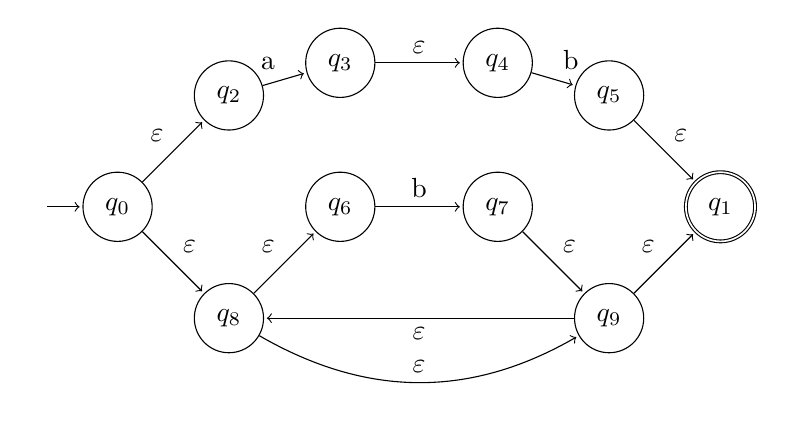
\begin{tikzpicture}[shorten >=1pt,node distance=2cm,on grid, auto,initial text=]
		\node[state,initial]	(q_0)												{$q_0$};
		
		\node[state]			(q_2)	[above right=of q_0]						{$q_2$};
		\node[state]			(q_3)	[above right=of q_2, yshift=-1cm]						{$q_3$};
		\node[state]			(q_4)	[right=of q_3]								{$q_4$};
		\node[state]			(q_5)	[below right=of q_4, yshift=1cm]						{$q_5$};
		\node[state]			(q_8)	[below right=of q_0]						{$q_8$};
		\node[state]			(q_6)	[above right=of q_8]						{$q_6$};
		\node[state]			(q_7)	[right=of q_6]								{$q_7$};
		\node[state]			(q_9)	[below right=of q_7]						{$q_9$};
		
		\node[state,accepting]	(q_1)	[above right=of q_9,below right=of q_5]		{$q_1$};
		
		\path[->]	(q_0)	edge	node	{$\varepsilon$}	(q_2)
							edge 	node	{$\varepsilon$} (q_8)
					(q_2)	edge	node	{a}				(q_3)
					(q_3)	edge	node	{$\varepsilon$}	(q_4)
					(q_4)	edge	node	{b}				(q_5)
					(q_5)	edge	node	{$\varepsilon$}	(q_1)
					
					(q_8)	edge	node	{$\varepsilon$}	(q_6)
							edge [bend right] node	{$\varepsilon$}	(q_9)
					(q_6)	edge	node	{b}				(q_7)
					(q_7)	edge	node	{$\varepsilon$}	(q_9)
					(q_9)	edge	node	{$\varepsilon$}	(q_8)
							edge	node	{$\varepsilon$}	(q_1);
	\end{tikzpicture}
	\caption{Diagram of a $\varepsilon$-NFA built using Thompson's construction for the regular expression $(ab + b^*)$.}
	\label{fig:nfa_thompson_example}
\end{figure}


%Thompson's construction is a classic algorithm for converting a regular expression into a nondeterministic finite automaton (NFA) with $\varepsilon$-transitions. It was introduced in 1968 by Ken Thompson and is the foundation for many regex engines, including the \texttt{lex} lexical analyzer generator.
%
%The construction proceeds recursively based on the structure of the regular expression. Each base case (such as a single symbol or the  $\varepsilon$) and each operator (`+`, concatenation, `*`) corresponds to a small NFA fragment. These fragments are then joined using $\varepsilon$-transitions.
%
%Although Thompson's NFA may contain many $\varepsilon$-transitions, it is guaranteed to be of size linear in the length of the regular expression. The resulting NFA can be converted into a deterministic finite automaton (DFA) using the standard powerset construction, typically after removing $\varepsilon$-transitions.

\subsection{Brzozowski's Derivatives}
In 1964, Brzozowski \cite{brzozowski_derivatives} proposed a method of constructing deterministic finite automata using derivatives, where consequent derivations of a regular expression would result in the states and their transitions with respect to the symbol derived.

\begin{defn}[Brzozowski's Automaton \cite{brzozowski_derivatives}]
	Let $\alpha \in \textbf{RegExp}$ be a regular expression defined over $\Sigma$. Brzozowski's automaton for the regular expression $\alpha$ is defined as the deterministic finite automaton $\mathcal{D} = (Q, \Sigma, q_0, \delta, F)$. $Q$ is the set of all dissimilar derivatives of $\alpha$, $q_0$ is the initial state ($q_0 \in Q$), $\delta$ is the transition function defined by $\delta: Q \times \Sigma \rightarrow Q$ such that $\delta (q,a) = d_a(q)$ for all $a \in \Sigma$ and $q \in Q$, and the set of final states is $F = \{q \in Q \, | \, \varepsilon(q) = \varepsilon\}$.
\end{defn}

For instance, let $\alpha = (ad+d^*)db$ over $\Sigma = \{a,b,d\}$. The transition function $\delta$ is defined for a Brzozowski's automaton $\mathcal{D}$ of $\alpha$ as:

\medspace $\alpha = (ad+d^*)db$:
\begin{align*}
	\delta((ad + d^*)db, a) &= d_a((ad + d^*)db) \\
	&= d_a(addb + d^*db) \\
	&= d_a(addb) + d_a(d^*db) \\
	&= d_a(a)ddb + \emptyset + \emptyset \\
	&= \varepsilon ddb
\end{align*}
\begin{align*}
	\delta((ad + d^*)db, b) &= d_b((ad + d^*)db) \\
	&= d_b(addb + d^*db) \\
	&= d_b(addb) + d_b(d^*db) \\
	&= \emptyset + \emptyset = \emptyset
\end{align*}
\begin{align*}
	\delta((ad + d^*)db, d) &= d_d((ad + d^*)db) \\
	&= d_d(addb + d^*db) \\
	&= d_d(addb) + d_d(d^*db) \\
	&= \emptyset + d_d(d^*)db + d_d(db) \\
	&= d_d(d)d^*db + d_d(d)b + d_d(b) \\
	&= \varepsilon d^*db + \varepsilon b + \emptyset \\
	&= d^*db + b
\end{align*}

\medspace $\alpha = ddb$:
\begin{align*}
	\delta(ddb, a) &= d_a(ddb) \\
	&= d_a(d)db \\
	&= \emptyset
\end{align*}
\begin{align*}
	\delta(ddb, b) &= d_b(ddb) \\
	&= d_b(d)db \\
	&= \emptyset
\end{align*}
\begin{align*}
	\delta(ddb, d) &= d_d(ddb) \\
	&= d_d(d)db\\
	&= \varepsilon db \\
	&= db
\end{align*}

\medspace $\alpha = d^*db + b$:
\begin{align*}
	\delta(d^*db + b, a) &= d_a(d^*db + b) \\
	&= d_a(d^*db) + d_a(b) \\
	&= \emptyset + \emptyset = \emptyset
\end{align*}
\begin{align*}
	\delta(d^*db + b, b) &= d_b(d^*db + b) \\
	&= d_b(d^*db) + d_b(b) \\
	&= \emptyset + \varepsilon = \varepsilon
\end{align*}
\begin{align*}
	\delta(d^*db + b, d) &= d_d(d^*db + b) \\
	&= d_d(d^*db) + d_d(b) \\
	&= d_d(d^*)db + d_d(db) + \emptyset \\
	&= d_d(d)d^*db + d_d(d)b + d_d(b) \\
	&= \varepsilon d^*db + \varepsilon b + \emptyset = d^*db + b
\end{align*}

\medspace $\alpha = db$:
\begin{align*}
	\delta(db, a) &= d_a(db) \\
	&= d_a(d)b \\
	&= \emptyset
\end{align*}
\begin{align*}
	\delta(db, b) &= d_b(db) \\
	&= d_b(d)b \\
	&= \emptyset
\end{align*}
\begin{align*}
	\delta(db, d) &= d_d(db) \\
	&= d_d(d)b \\
	&= \varepsilon b = b
\end{align*}

\medspace $\alpha = b$
\begin{align*}
	\delta(b, a) &= d_a(b) \\
	&= \emptyset
\end{align*}
\begin{align*}
	\delta(b, b) &= d_b(b) \\
	&= \varepsilon
\end{align*}
\begin{align*}
	\delta(b, d) &= d_d(b) \\
	&= \emptyset
\end{align*}

Finally, the set of states for $\mathcal{D}$ is $Q = \{ (ad+d^*)db, ddb, d^*db + b, db, b, \varepsilon, \emptyset \}$ and the set of final states is $F = \{ \varepsilon \}$. The diagram for this automaton is shown in \ref{fig:brzozowski_derivatives_example}.

\begin{figure}[H]
	\centering
	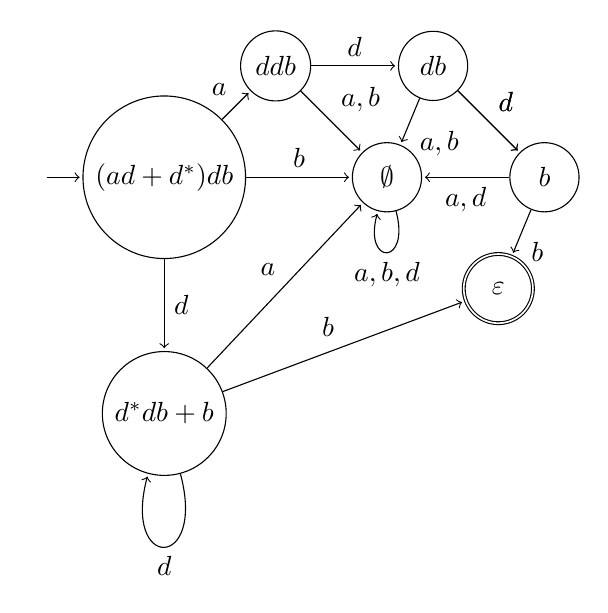
\begin{tikzpicture}[shorten >=1pt,node distance=2cm,on grid, auto,initial text=]
		\node[state,initial]	(q_0)												{$(ad+d^*)db$};
		\node[state]			(q_1)	[above right=of q_0]						{$ddb$};
		
		\node[state]			(q_3)	[right=of q_1]								{$db$};
		\node[state]			(q_4)	[below right=of q_3]						{$b$};
		\node[state]			(q_5)	[below right=of q_1]						{$\emptyset$};
		\node[state, accepting]	(q_6)	[below right=of q_5]						{$\varepsilon$};
		
		\node[state]			(q_2)	[below=30mm of q_0]							{$d^*db + b$};
		
		\path[->]	(q_0)	edge	node				{$a$}	(q_1)
							edge	node				{$d$}	(q_2)
							edge	node				{$b$}	(q_5)
					(q_1)	edge	node				{$d$}	(q_3)
							edge	node				{$a,b$}	(q_5)
					(q_2)	edge	node				{$a$}	(q_5)
							edge 	[loop below]	node	{$d$}	()
							edge	node				{$b$}	(q_6)
					(q_3)	edge	node				{$d$}	(q_4)
							edge	node				{$a,b$}	(q_5)
							edge	node				{$d$}	(q_4)
					(q_4)	edge	node				{$b$}	(q_6)
							edge	node				{$a,d$}	(q_5)
					(q_5)	edge	[loop below]	node	{$a,b,d$} ();
	\end{tikzpicture}
	\caption{Diagram of a Brzozowki DFA for the regular expression $(ad+d^*)db$.}
	\label{fig:brzozowski_derivatives_example}
\end{figure}

%This method can, however, lead to an exponential number of distinct derivatives in the worst case. Therefore, simplification rules and expression equivalences are critical to making the approach practical.

%\subsection{Antimirov's Partial Dertivatives}
%Proposed by Valery Antimirov in 1996 \cite{pdregex_antimirov}, the partial derivatives construction generalizes Brzozowski's derivatives to build an NFA rather than a DFA. Instead of producing a single derivative for each symbol, Antimirov's method produces a \emph{set} of partial derivatives, reflecting the inherent nondeterminism of the regular expression.
%
%This construction avoids $\varepsilon$-transitions and yields a compact $\varepsilon$-free NFA. Each partial derivative corresponds to a transition in the automaton, and the process naturally handles alternation and repetition.
%
%\begin{defn}[Partial Derivatives Automaton]
%	Let $\alpha \in RegExp$ over $\Sigma$. The partial derivatives automaton for $\alpha$ is defined as the non-deterministic finite automaton $\mathcal{N} = (Q_{\mathcal{PD}}, \Sigma, q_0, \delta, F)$. $q_0$ is the initial state and belongs to the set of states $Q_{\mathcal{PD}}$. It is important to note that $q_0 = \alpha$. The transition function is defined as $\delta(q,a) = \partial_a(q)$ for all symbols $a \in \Sigma$ and states $q \in Q_{\mathcal{PD}}$. The set of final states is defined as $F = \{ q \in Q_{\mathcal{PD}} \, | \, \varepsilon(q) = \varepsilon \}$.
%\end{defn}
%
%Recalling from \ref{chap:prelim:linear_form}, the linear form can be used as an efficient way to compute partial derivatives.
%Let $\alpha \in RegExp$ over $\Sigma$ and $a \in \Sigma$:
%\begin{centering}
%	$\delta(\alpha, a) = \{  \}$
%\end{centering}

\subsection{Antimirov's Partial Derivatives}
Proposed by Valery Antimirov in 1996 \cite{pdregex_antimirov}, the partial derivatives construction generalizes Brzozowski's derivatives to build an NFA rather than a DFA. Instead of producing a single derivative for each symbol, Antimirov's method produces a \emph{set} of partial derivatives, reflecting the inherent nondeterminism of the regular expression.

This construction avoids $\varepsilon$-transitions and yields a compact $\varepsilon$-free NFA. Each partial derivative corresponds to a transition in the automaton, and the process naturally handles alternation and repetition.


\begin{defn}[Partial Derivatives Automaton]
	Let $\alpha \in RegExp$ over $\Sigma$. The partial derivatives automaton for $\alpha$ is defined as the non-deterministic finite automaton $\mathcal{N} = (Q_{\mathcal{PD}}, \Sigma, q_0, \delta, F)$. $q_0$ is the initial state and belongs to the set of states $Q_{\mathcal{PD}}$. It is important to note that $q_0 = \alpha$. The transition function is defined as $\delta(q,a) = \partial_a(q)$ for all symbols $a \in \Sigma$ and states $q \in Q_{\mathcal{PD}}$. The set of final states is defined as $F = \{ q \in Q_{\mathcal{PD}} \, | \, \varepsilon(q) = \varepsilon \}$.
\end{defn}

Recalling from \ref{chap:prelim:linear_form}, the linear form can be used as an efficient way to compute partial derivatives.
Let $\alpha \in RegExp$ over $\Sigma$ and $a \in \Sigma$:
\[
\delta(\alpha, a) = \partial_a(\alpha) = \{ \beta \mid (a,\beta) \in lf(\alpha) \}.
\]

That is, to compute the set of partial derivatives of $\alpha$ with respect to a symbol $a$, one inspects the linear form of $\alpha$ and collects all continuations $\beta$ that follow an $a$ in the prefix position. This characterization is not only concise but also algorithmically useful: it gives a direct recipe for building the transition relation of the partial derivatives automaton.

\begin{thm}[\cite{pdregex_antimirov}]
	For every regular expression $\alpha$, the partial derivatives automaton $\mathcal{N}_\alpha$ accepts exactly the language $L(\alpha)$. Moreover, the number of states of $\mathcal{N}_\alpha$ is bounded by $|\alpha|+1$.
\end{thm}

%For instance, let $\alpha = (ad+d^*)db$ over $\Sigma = \{a,b,d\}$. The set of 


\subsection{Position Automata}
%https://www.dcc.fc.up.pt/~nam/resources/publica/dlt16.pdf

% To first recall the notion of \emph{position automata} (also known as \emph{Glushkov automata}), one must first understand the idea of marking each occurrence of a symbol in a regular expression with a unique position. This transforms a regular expression into a \emph{marked regular expression}, where each letter is indexed according to its position in the expression when read left to right. The position automaton is then constructed from this marked version by associating each position with a distinct state, and defining transitions based on the structural analysis of the expression.

The \emph{position automaton}, also known as the \emph{Glushkov automaton}, is a type of $\varepsilon$-free nondeterministic finite automaton (NFA) constructed directly from a regular expression. Unlike the standard Thompson construction, which introduces $\varepsilon$-transitions that must later be eliminated, the Glushkov construction yields an automaton in which each state corresponds uniquely to a symbol occurrence---or \emph{position}---in the expression. \cite{mesh-of-automata}

Given a regular expression $E$, the Glushkov automaton $M_E$ is defined based on three key position-based functions:

\begin{itemize}
    \item \textbf{first$(E)$}: the set of positions that can appear first in some word of the language $\mathcal{L}(E)$.
    \item \textbf{last$(E)$}: the set of positions that can appear last in some word of $\mathcal{L}(E)$.
    \item \textbf{follow$(E, x)$}: for each position $x$, the set of positions that can immediately follow $x$ in some word of $\mathcal{L}(E)$.
\end{itemize}

To distinguish different occurrences of the same symbol, the construction introduces marked symbols. For example, the expression $(a + b)^*a(b + a)^*$ is rewritten as $(a_1 + b_2)^*a_3(b_4 + a_5)^*$. Each marked symbol corresponds to a unique position and becomes a distinct state in the automaton.

The Glushkov automaton $M_E = (Q, \Sigma, \delta, q_0, F)$ is constructed as follows:

\begin{itemize}
    \item $Q$ is the set of positions in $E$ (i.e., the marked symbols), plus an initial state $q_0$.
    \item For each symbol $a \in \Sigma$:
    \begin{itemize}
        \item $\delta(q_0, a) = \{ x \in \text{first}(E) \mid \text{symbol}(x) = a \}$
        \item $\delta(x, a) = \{ y \in \text{follow}(E, x) \mid \text{symbol}(y) = a \}$
    \end{itemize}
    \item The set of final states $F$ is $\text{last}(E)$; if $\varepsilon \in \mathcal{L}(E)$, then $q_0$ is also final.
\end{itemize}

This automaton captures the structural flow of $E$ by tracing symbol sequences as state transitions. It is $\varepsilon$-free and has one state per symbol occurrence, which results in at most a quadratic number of transitions with respect to the size of $E$.

An important property of the Glushkov automaton is its relationship to unambiguity. A regular expression is \emph{weakly unambiguous} if and only if its Glushkov automaton is unambiguous, i.e., there exists at most one accepting path for each accepted word. This makes the Glushkov construction a practical and efficient tool in applications requiring unambiguous parsing, such as syntax analysis in document type definitions (e.g., SGML and XML DTDs).



% The key to this construction lies in the inductive computation of three sets: \emph{First}, \emph{Last}, and \emph{Follow}.The \emph{First} set contains positions that may begin a word in the language; the \emph{Last} set includes positions that may end such words; and the \emph{Follow} relation determines which positions can immediately follow a given position in any word generated by the expression. The resulting automaton has states corresponding to positions, transitions derived from the \emph{Follow} relation, an initial state representing position 0 (the start of matching), and final states determined by the \emph{Last} set, extended with position 0 if the empty string is accepted. \cite{mesh-of-automata}


\section{FAdo}
The FAdo \cite{fado_paper} project is an open-source implementation of several sets of tools for formal languages manipulation. In order to allow quick prototyping and testing of algorithms, these tools were developed in Python. Regular languages can be represented by regular expressions which are defined in \texttt{reex.py} - or by finite automata which are defined in \texttt{fa.py}.

\subsection{Finite Automata}

\begin{figure}[H]
	\centering
	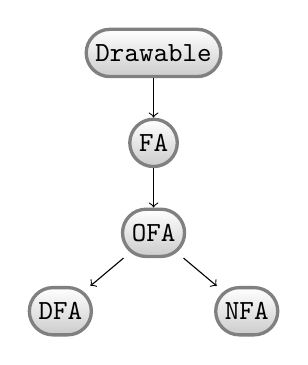
\begin{tikzpicture}[node distance=5mm,
		terminal/.style={
			% The shape:
			rectangle,minimum size=6mm,rounded corners=3mm,
			% The rest
			very thick,draw=black!50,
			top color=white,bottom color=black!20,
			font=\ttfamily}]
		\node (c_dwble)		[terminal]                {Drawable};
		\node (c_fa)		[terminal, below=of c_dwble]   {FA};
		\node (c_ofa)		[terminal, below=of c_fa] {OFA};
		\node (c_nfa)		[terminal, below right=of c_ofa] {NFA};
		\node (c_dfa)		[terminal, below left=of c_ofa]{DFA};
		
		\path	(c_dwble)	edge[->]	(c_fa)
				(c_fa)		edge[->]	(c_ofa)
				(c_ofa)		edge[->]	(c_dfa)
							edge[->]	(c_nfa);
	\end{tikzpicture}
	\caption{Class inheritance organization in FAdo's finite automata code file, \texttt{fa.py} (excluding the \texttt{SemiDFA} class)}
	\label{fig:fado_fa_diag}
\end{figure}

%As shown in \ref{fig:fado_fa_diag}, \texttt{FAdo}'s FA implementation utilizes the base class \texttt{Drawable} all the other children classes. The \texttt{Drawable} class will only set up some basic methods and properties used to draw the automata with the help of the \texttt{graphviz} library.
%The \textt{}


As shown in Figure~\ref{fig:fado_fa_diag}, FAdo organizes its implementation of finite automata as an inheritance hierarchy. At the top level, the class \texttt{Drawable} provides only drawing functionality, relying on the \texttt{graphviz} backend to visualize automata.

On top of this, the class \texttt{FA} defines the abstract interface for finite automata, introducing the fundamental components: the set of states, the alphabet, the transition function, the initial state(s), and the set of final states. This class also establishes common methods for manipulating these elements and for interoperability between automata.

The class \texttt{OFA} (``one-way finite automaton'') specializes \texttt{FA} and serves as the immediate superclass for concrete models. It defines abstract operations such as evaluation of symbols, addition of transitions, and access to useful states, ensuring a consistent contract across different automaton types.

Two subclasses will then inherit from \texttt{OFA}:
\begin{itemize}
	\item \texttt{NFA} --- implements nondeterministic finite automata, possibly with $\varepsilon$-transitions. It provides methods for epsilon-closure, elimination of $\varepsilon$-moves, subset construction into a DFA, and regular operations such as union, concatenation, and Kleene star.
	\item \texttt{DFA} --- implements deterministic finite automata. It enforces determinism by construction and provides efficient word evaluation and minimization routines.
\end{itemize}

\subsection{Regular Expressions}
In \texttt{reex.py}, FAdo defines the \texttt{RegExp} base class for all regular expressions, declaring therein a class variable \texttt{sigma}, formally known as the set of symbols ($\Sigma$).
To represent any and all base constructions of a regular expressions, FAdo defines base classes for each of them:
\begin{itemize}
    \item \textbf{CEmptySet}: The empty symbol set. ($\emptyset$)
    \item \textbf{CEpsilon}: The empty string. ($\varsigma$)
    \item \textbf{CAtom}: A simple symbol. (e.g. $'a'$)
    \item \textbf{CDisj}: The $+$ operation between symbols. (e.g. \texttt{CDisj(CAtom(a),CAtom(b))} represents the regular expression $R=a+b$ where $a,b \in \Sigma_R$)
    \item \textbf{CConcat}: The $\cdot$ operation 
    \item \textbf{CStar}: The Kleene closure over a set of symbols (e.g. \texttt{CStar(CDisj(CAtom(a),CAtom(b)))} representes the regular expression $R=(a+b)^*$ where $a,b \in \Sigma_R$)

\end{itemize}

In order to parse expressions into FAdo's classes and types, \emph{lark} was used. \emph{lark} is a parsing toolkit for Python. It can parse all context-free languages.





%\chapter{State of the Art}\label{chap:art}
\chapter{State of the Art}\label{chap:art}

\section{Overview of XYZ}
%%%%%%%%%%%%%%%%%%%%%%%%%%%%%%%%%%%%%%%%
Computers are devices that



%\chapter{Desenho da Arquitetura}\label{chap:syst}
\chapter{Matching}\label{chap:devel}

The implementation chapter gives insights into 

\section{Normal Matching}
\subsection{Standard Matching}

\subsection{Greedy Matching}


\section{Multi Matching}



%\chapter{Resultados e análise}\label{chap:results}
% !TEX root = thesis.tex

\chapter{Results and Discussion}\label{chap:results}

This is a test

\section{Evaluation}

The methods of evaluating
 

%\chapter{Conclusões}\label{chap:conc}
\chapter{Conclusion}
In this work, we contribute with a new approach to address the problem of \ac{ReDoS}, focusing on a solution outside of traditional backtracking engines.
We explored the underlying causes of ReDoS vulnerabilities, particularly how certain finite automaton evaluators can lead to catastrophic performance, due to the deviation of the path of theory. To tackle this, we extended \textit{FAdo} to support fixed and bounded repetition operators. To recognize this new grammar, the default Lark grammar present in \textit{FAdo} was modified. The new type of automaton is capable of performing multiple overlapping matching.
Overall, this work contributes towards safer and more predictable regular expression evaluation by combining formal methods and a new matching strategy.

Future work may turn towards making these algorithms more efficient by switching to a different language or integrating them into a larger ecosystem. It would also be very interesting to develop a tool that generates overlapped text datasets

%With this, a new type of automaton was implemented and used to perform multiple overlapping matching.



%% references
%\renewcommand{\bibname}{Referências} % o babel portuguese coloca Bibliografia
% os meses do ficheiro bib poderão aparecer em inglês, caso se pretenda deve-se colocar o texto em português explicitamente no ficheiro bid
\cleardoublepage%
\phantomsection%
\printbibliography[heading=bibintoc]%


%% appendix
\appendix
\include{appendix1}

%% bye
\end{document}
